\section{抛物线}

\subsection{抛物线的单点设法}

\begin{theorem}
    抛物线 $y^2=4x$ 上的一个动点，可以设它的坐标为 $(\frac{t^2}{4},t)$，（仅一个变量），而椭圆、双曲线只能设为 $(x_0,y_0)$.
\end{theorem}

\begin{example}
    如图，O为坐标原点，F为抛物线 C: $y^2=8x$ 的焦点，P为C上一点，若 $|PF|=8$，则 $\triangle POF$ 的面积为 ( \quad )
\end{example}

\v{1em}

\begin{minipage}[c]{0.5\textwidth}
    \centering
    \begin{tikzpicture}[scale=0.7]
        \begin{axis}[
                axis lines=middle,
                xlabel=$x$,
                ylabel=$y$,
                xmin=-1, xmax=9,
                ymin=-8, ymax=8,
                xtick={2},
                xticklabels={F(2,0)},
                ytick=\empty,
                enlargelimits=false,
            ]
            % 抛物线
            \addplot[domain=0:9, samples=100, thick, blue] {sqrt(8*x)};
            \addplot[domain=0:9, samples=100, thick, blue] {-sqrt(8*x)};
            % 点P的坐标
            \pgfmathsetmacro{\xP}{4}
            \pgfmathsetmacro{\yP}{sqrt(8*\xP)}
            % 点和标签
            \node[below left] at (0,0) {O};
            \node[above right] at (\xP, \yP) {$P(x_0, y_0)$};
            \fill (\xP, \yP) circle (2pt);
            % 三角形
            \draw[thick] (0,0) -- (\xP, \yP) -- (2,0) -- cycle;
        \end{axis}
        % 手写笔记
        \node[right, color=blue] at (4.5, 4) {$\begin{aligned}P(\frac{y_0^2}{8}, y_0)\end{aligned}$};
        \node[right, color=blue, scale=0.9] at (7, 3) {$\sqrt{(\frac{y_0^2}{8}-2)^2 + y_0^2}=8$};
    \end{tikzpicture}
\end{minipage} %
\begin{minipage}[c]{0.5\textwidth}
    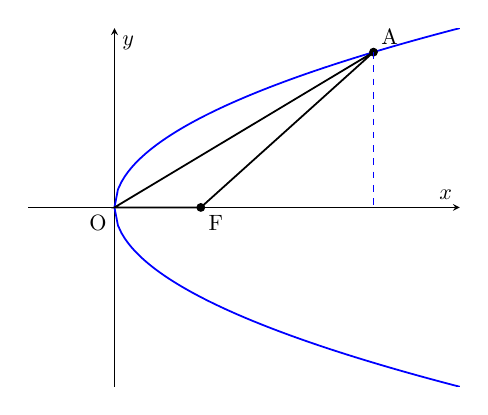
\begin{tikzpicture}[scale=0.8]
        \begin{axis}[
                axis lines=middle,
                xlabel=$x$,
                ylabel=$y$,
                xmin=-1, xmax=4,
                ymin=-4, ymax=4,
                xtick=\empty,
                ytick=\empty,
                enlargelimits=false,
            ]
            % 抛物线 y^2=4x
            \addplot[domain=0:4, samples=100, thick, blue] {sqrt(4*x)};
            \addplot[domain=0:4, samples=100, thick, blue] {-sqrt(4*x)};
            % 点和标签
            \coordinate (O) at (0,0);
            \coordinate (F) at (1,0);
            \coordinate (A) at (3, {2*sqrt(3)});
            \node[below left] at (O) {O};
            \node[below right] at (F) {F};
            \node[above right] at (A) {A};
            \fill (A) circle (2pt);
            \fill (F) circle (2pt);
            % 三角形
            \draw[thick] (O) -- (A) -- (F) -- cycle;
            % 辅助线
            \draw[dashed, blue] (A) -- (3,0);
        \end{axis}
    \end{tikzpicture}
\end{minipage}

\v{1em}

\begin{problem}
$y^2=2px(p>0)$ 焦点为 $F(1,0)$，A 在抛物线上，O 是原点，若 $\triangle OFA$ 的面积为 $\sqrt{3}$，则 $\angle OFA = ( \quad )$
\end{problem}

\vspace{2em}

\begin{problem}
设 P 是抛物线 $y^2=-4 x$ 上一点，则点 P 到椭圆 $\frac{x^2}{16}+\frac{y^2}{15}=1$ 的左顶点的距离的最小值为 \underline{\hspace{2em}}.
\end{problem}

\v{2em}

\begin{problem}
设抛物线 $C: y^2=2px(p>0)$ 的焦点为 F, P为抛物线C上任意一点，O为坐标原点，M为线段FP的中点，则直线OM斜率的最大值为 ( \quad )
\begin{tasks}(4)
    \task $\frac{1}{2}$
    \task 1
    \task $\frac{p}{2}$
    \task p
\end{tasks}
\end{problem}

\v{2em}

\begin{example}
    设点 $P$ 是抛物线 $C: y^2=4 x$ 上一动点，$F$ 是抛物线的焦点，$O$ 为坐标原点，则 $\frac{|O P|}{|P F|}$ 的最大值为 $\qquad$
\end{example}

\vspace{6em}

\begin{example}
    抛物线 $C: y^2=4 x$ 的焦点为 $F$ ，动点 $P$ 在抛物线 $C$ 上，点 $A(-1,0)$ ，当 $\frac{|P A|}{|P F|}$ 取得最大值时，直线 $A P$ 的方程为 $\qquad$
\end{example}

\v{8em}

\subsection{抛物线和直线的联立}

\begin{example}
    点 $F$ 为抛物线 $C: y^2=4 x$ 的焦点，过 $F$ 的直线 $l$ 与 $C$ 交于 $A, B$ 两点，则 $|A F|+2|B F|$ 的最小值为（ \hspace{2em}）
    \begin{tasks}(4)
        \task $2 \sqrt{2}$
        \task 4
        \task $3+2 \sqrt{2}$
        \task 6
    \end{tasks}
\end{example}

\begin{example}
    直线 $l: x-2 y+2=0$ 与抛物线 $C: y^2=4 x$ 相交于 $A, B$ 两点，则 $\overrightarrow{O A} \cdot \overrightarrow{O B}$ 的值为（\hspace{2em} ）
    \begin{tasks}(4)
        \task 4
        \task 8
        \task 12
        \task 16
    \end{tasks}
\end{example}

\begin{example}
    抛物线 $C: y^2=4 x$ 的焦点为 $F$ ，准线为 $l$ ，点 $P$ 为 $C$ 上一点，过点 $P$ 作 $l$ 的垂线，垂足为 $A$ ，若 $\overrightarrow{F A}=2 \overrightarrow{F B}$ ，且点 $(-3,0)$ 在直线 $P B$ 上，则直线 $P B$ 的斜率为（ \hspace{2em}）
    \begin{tasks}(4)
        \task $\frac{\sqrt{3}}{6}$ 或 $-\frac{\sqrt{3}}{6}$
        \task $\frac{\sqrt{3}}{3}$ 或 $-\frac{\sqrt{3}}{3}$
        \task 1或 -1
        \task $\sqrt{3}$ 或 $-\sqrt{3}$
    \end{tasks}
\end{example}

\subsection{二级结论}

\begin{definition}
    如图，$\triangle A H B$ 称为阿基米德三角形。

    设：$A\left(x_1, y_1\right) 、 B\left(x_2, y_2\right), A B$ 中点 $G\left(x_0, y_0\right)$ ，直线 $A B: x=t y+\frac{p}{2}$ ．则：
\end{definition}

\begin{figure} [H]
    \centering
    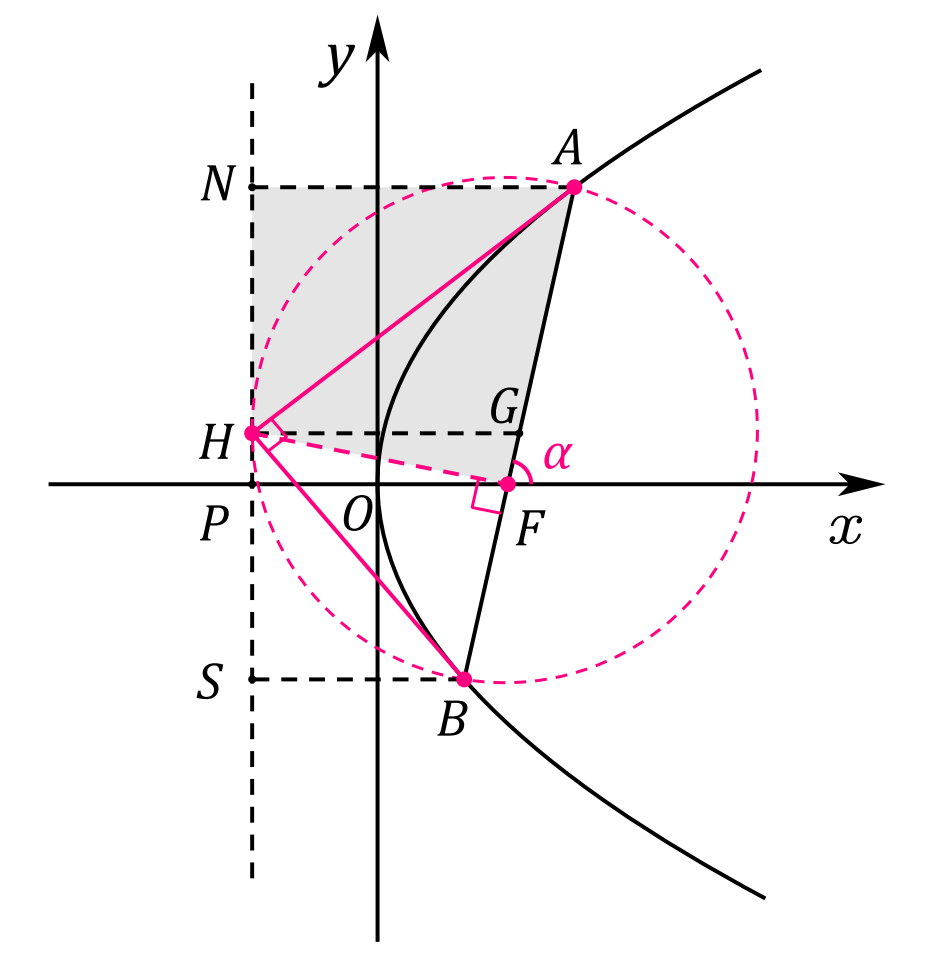
\includegraphics[width=0.3\textwidth]{chapters/圆锥曲线/images/抛物线/img-20250605220316.png}
\end{figure}

\begin{theorem}

    （1）第一焦半径公式：$|A F|=|A N|=x_1+\frac{p}{2}$ ，即：$|A F|=x_1+\frac{p}{2}$ ，同理有：$|B F|=x_2+\frac{p}{2}$.

    $$|A B|=|A F|+|B F|=x_1+x_2+p=2\left(x_0+\frac{p}{2}\right)$$

    （2）第二焦半径公式：设直线 $A B$ 的倾斜角为 $\alpha$ ，则有：$|A F|=\frac{p}{1-\cos \alpha}$、$|B F|=\frac{p}{1+\cos \alpha}$（长减短加）

    $$|A B|=|A F|+|B F|=\frac{2 p}{1-\cos ^2 \alpha}=\frac{2 p}{\sin ^2 \alpha}=2 p\left(1+\frac{1}{k^2}\right)$$

    $$\frac{1}{|F A|}+\frac{1}{|F B|}=\frac{1-\cos \alpha}{p}+\frac{1+\cos \alpha}{p}=\frac{2}{p}$$

    （3）抛物线的坐标平均性：$\left\{\begin{array}{l}x=t y+\frac{p}{2} \\ y^2=2 p x\end{array} \Longrightarrow y^2-2 p t y-p^2=0 \Longrightarrow\left\{\begin{array}{l}y_1 y_2=-p^2 \\ x_1 x_2=\frac{p^2}{4}\end{array}\right.\right.$

    （4）$\because G$ 到准线距离 $d=x_0+\frac{p}{2}=\frac{1}{2}|A B|$ ，可知：以 $A B$ 为直径的圆与准线 $l$ 相切

    （5）$\angle H A G=\angle A H G \Longrightarrow\left\{\begin{array}{l}\triangle A N H \cong \triangle A H F \Longrightarrow F H \perp A B \\ G H / / A N / / S B / / x \text { 轴 }\end{array}\right.$

    （6）$H A$、$H B$ 为抛物线的两条切线
\end{theorem}

\begin{example}
    点 $F$ 为抛物线 $C: y^2=4 x$ 的焦点，过 $F$ 的直线 $l$ 与 $C$ 交于 $A, B$ 两点，则 $|A F|+2|B F|$ 的最小值为（ \hspace{2em}）
    \begin{tasks}(4)
        \task $2 \sqrt{2}$
        \task 4
        \task $3+2 \sqrt{2}$
        \task 6
    \end{tasks}
\end{example}

The Maxwell's equations in differential form are:
\begin{align}
    \nabla \cdot \mathbf{B} = 0
\end{align}